\subsection{Caso d'uso UC5: Gestione profilo utente}
\begin{center}
	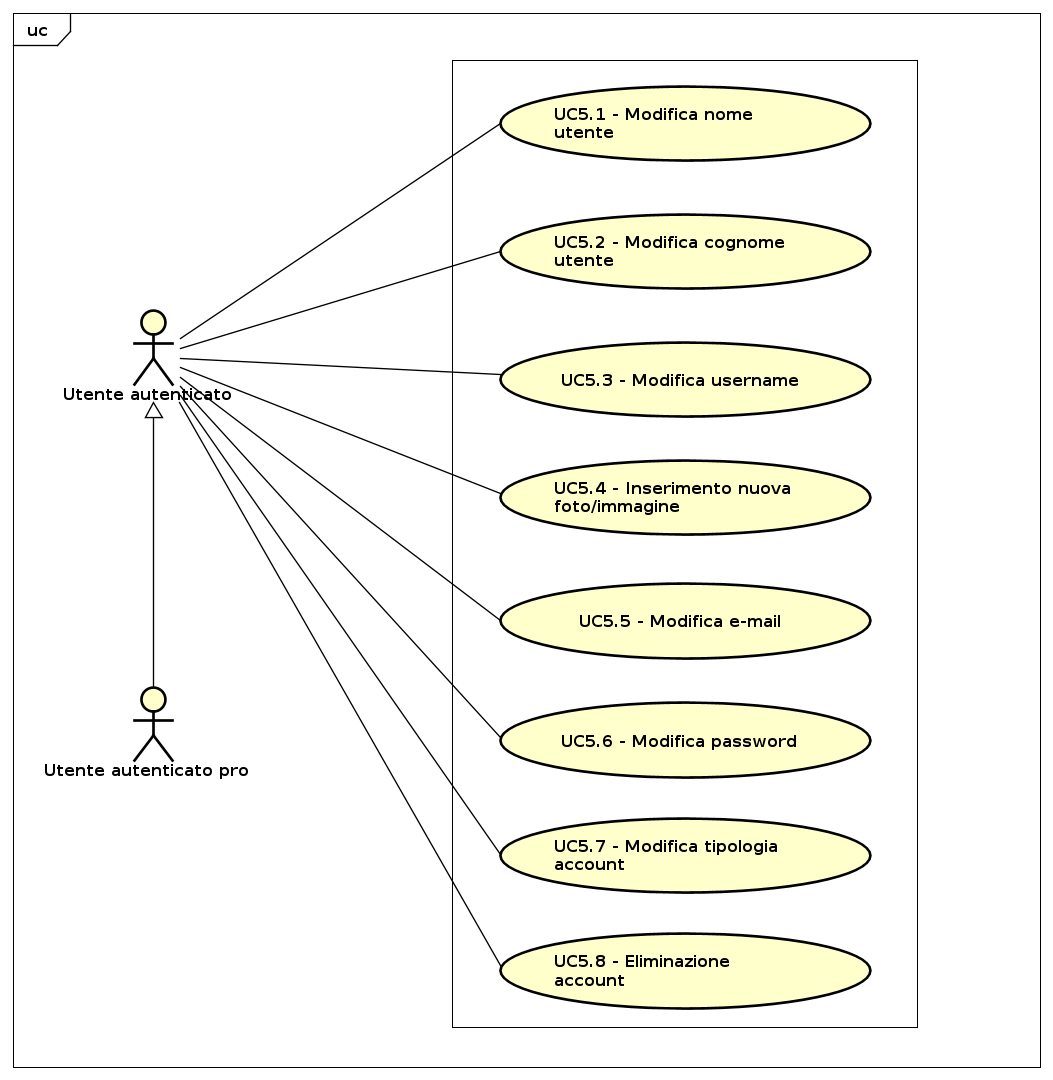
\includegraphics[scale=0.5]{UML/UC5.png}
\end{center}
\begin{itemize}
	\item \textbf{Attori}: utente autenticato;
	\item \textbf{Descrizione}: l'utente autenticato può visualizzare e modificare i suoi dati personali;
	\item \textbf{Precondizione}: il sistema è predisposto per consentire all'utente autenticato di gestire i propri dati personali;
	\item \textbf{Postcondizione}: il sistema ha attuato le modifiche effettuate dall'utente autenticato ai propri dati personali;
	\item \textbf{Scenario principale}:
		\begin{enumerate}
			\item L'utente autenticato può modificare il proprio nome utente (UC5.1);
			\item L'utente autenticato può modificare la propria e-mail (UC5.2);
			\item L'utente autenticato può modificare la propria password (UC5.3);
			\item L'utente autenticato può eliminare il proprio account (UC5.4).
		\end{enumerate} 
	\item \textbf{Scenari alternativi}: se le operazioni di modifica non vengono confermate il sistema non le rende persistenti e visualizza le funzionalità di gestione del profilo utente. 
\end{itemize}

\subsubsection{Caso d'uso UC5.1: Modifica nome utente}
\begin{center}
	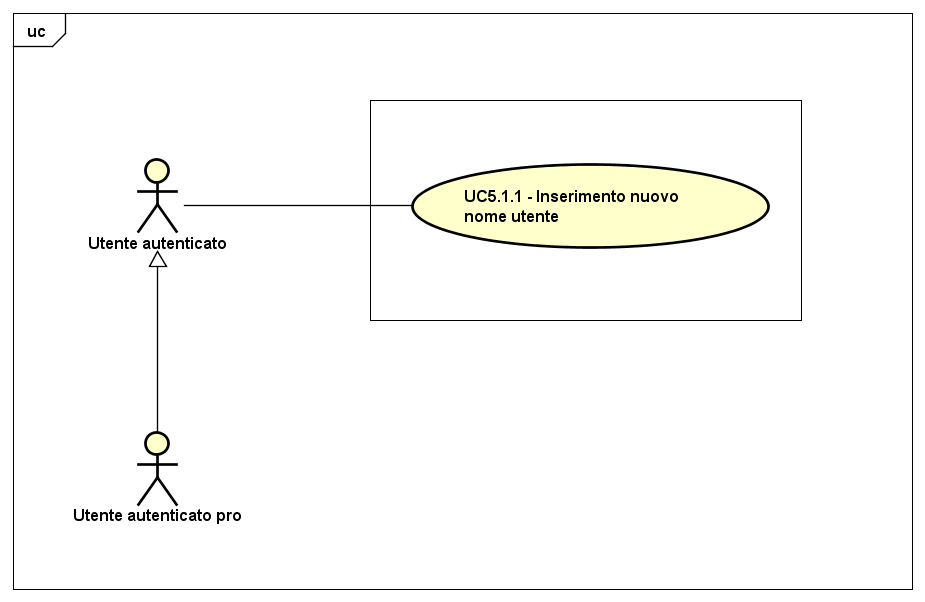
\includegraphics[scale=0.5]{UML/UC5_1.png}
\end{center}

\begin{itemize}
	\item \textbf{Attori}: utente autenticato;
	\item \textbf{Descrizione}: l'utente autenticato può modificare il proprio nome e cognome utente;
	\item \textbf{Precondizione}: il sistema presenta la schermata dove è possibile modificare nome e cognome utente;
	\item \textbf{Postcondizione}: il sistema ha reso persistenti le modifiche al nome e cognome utente;
	\item \textbf{Scenario principale}:
		\begin{enumerate}
			\item L'utente autenticato può inserire un nuovo nome utente (UC5.1.1);
			\item L'utente autenticato può inserire un nuovo cognome utente (UC5.1.2);
			\item L'utente autenticato può confermare le modifiche al nome e cognome utente (UC5.1.3).
		\end{enumerate}
	\item \textbf{Scenari alternativi}: l'utente autenticato annulla le modifiche e il sistema lo riporta alla schermata di gestione del profilo utente.
\end{itemize}

\paragraph{Caso d'uso UC5.1.1: Inserimento nuovo nome utente}

\begin{itemize}
	\item \textbf{Attori}: utente autenticato;
	\item \textbf{Descrizione}: l'utente autenticato può inserire un nuovo nome utente;
	\item \textbf{Precondizione}: il sistema richiede all'utente autenticato di inserire un nuovo nome utente;
	\item \textbf{Postcondizione}: l'utente autenticato ha inserito il nuovo nome utente;
	\item \textbf{Scenario principale}: l'utente autenticato inserisce il nuovo nome utente.
\end{itemize}

\paragraph{Caso d'uso UC5.1.2: Inserimento nuovo cognome utente}

\begin{itemize}
	\item \textbf{Attori}: utente autenticato;
	\item \textbf{Descrizione}: l'utente autenticato può inserire un nuovo cognome utente;
	\item \textbf{Precondizione}:  il sistema richiede all'utente autenticato di inserire un nuovo cognome utente;
	\item \textbf{Postcondizione}:  l'utente autenticato ha inserito il nuovo cognome utente;
	\item \textbf{Scenario principale}: l'utente autenticato inserisce il nuovo cognome utente.
\end{itemize}

\paragraph{Caso d'uso UC5.1.3: Conferma modifiche nome e cognome utente}

\begin{itemize}
	\item \textbf{Attori}: utente autenticato;
	\item \textbf{Descrizione}: l'utente autenticato può confermare le modifiche al proprio nome e cognome utente;
	\item \textbf{Precondizione}: l'utente ha inserito nuovi nome e cognome utente;
	\item \textbf{Postcondizione}: il sistema rende persistenti le modifiche effettuate al nome e cognome utente;
	\item \textbf{Scenario principale}: l'utente conferma le modifiche al nome e cognome utente.
\end{itemize}

\subsubsection{Caso d'uso UC5.2: Modifica e-mail}
\begin{center}
	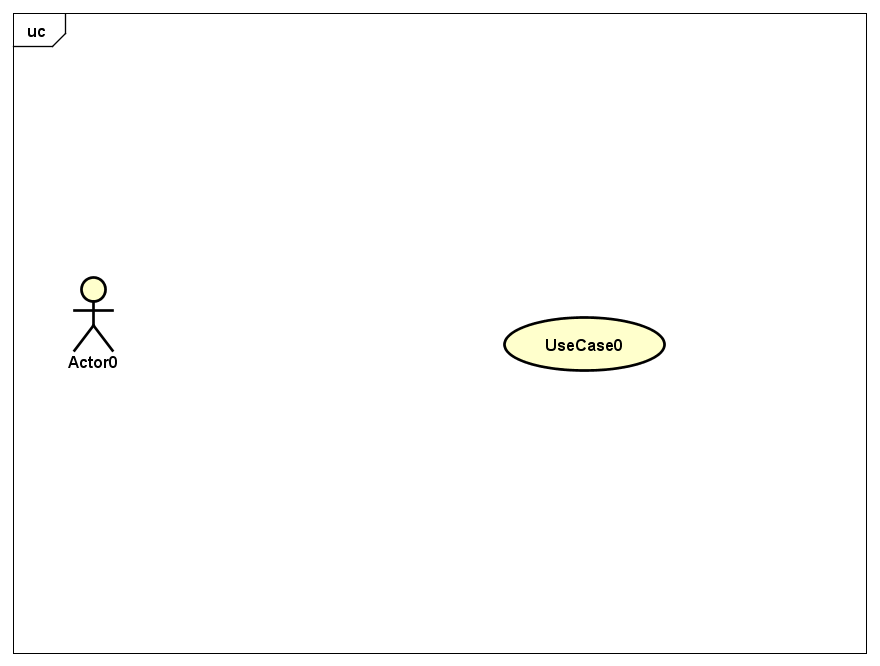
\includegraphics[scale=0.5]{UML/UC5_2.png}
\end{center}

\begin{itemize}
	\item \textbf{Attori}: utente autenticato;
	\item \textbf{Descrizione}: l'utente autenticato può modificare il proprio indirizzo di posta elettronica inserendone uno nuovo;
	\item \textbf{Precondizione}: il sistema presenta la schermata dove è possibile modificare l'indirizzo di posta elettronica;
	\item \textbf{Postcondizione}: il sistema ha reso persistenti le modifiche all'indirizzo di posta elettronica;
	\item \textbf{Scenario principale}:
		\begin{enumerate}
			\item L'utente autenticato può inserire un nuovo indirizzo di posta elettronica (UC5.2.1);
			\item L'utente autenticato può confermare le modifiche al proprio indirizzo di posta elettronica (UC5.2.2).
		\end{enumerate}
	\item \textbf{Scenari alternativi}: l'utente autenticato annulla le modifiche e il sistema lo riporta alla schermata di gestione del profilo utente.
\end{itemize}

\paragraph{Caso d'uso UC5.2.1: Inserimento nuova e-mail}

\begin{itemize}
	\item \textbf{Attori}: utente autenticato;
	\item \textbf{Descrizione}: l'utente autenticato può inserire un nuovo indirizzo di posta elettronica;
	\item \textbf{Precondizione}: il sistema richiede all'utente autenticato di inserire un nuovo indirizzo di posta elettronica;
	\item \textbf{Postcondizione}: l'utente autenticato ha inserito un nuovo indirizzo di posta elettronica;
	\item \textbf{Scenario principale}: l'utente autenticato inserisce un nuovo indirizzo di posta elettronica.
\end{itemize}

\paragraph{Caso d'uso UC5.2.2: Conferma modifiche e-mail}

\begin{itemize}
	\item \textbf{Attori}: utente autenticato;
	\item \textbf{Descrizione}: l'utente autenticato può confermare le modifiche al proprio indirizzo di posta elettronica;
	\item \textbf{Precondizione}: l'utente ha inserito un nuovo indirizzo di posta elettronica;
	\item \textbf{Postcondizione}: il sistema rende persistenti le modifiche effettuate all'indirizzo di posta elettronica;
	\item \textbf{Scenario principale}: l'utente conferma le modifiche all'indirizzo di posta elettronica.
\end{itemize}

\subsubsection{Caso d'uso UC5.3: Modifica password}
\begin{center}
	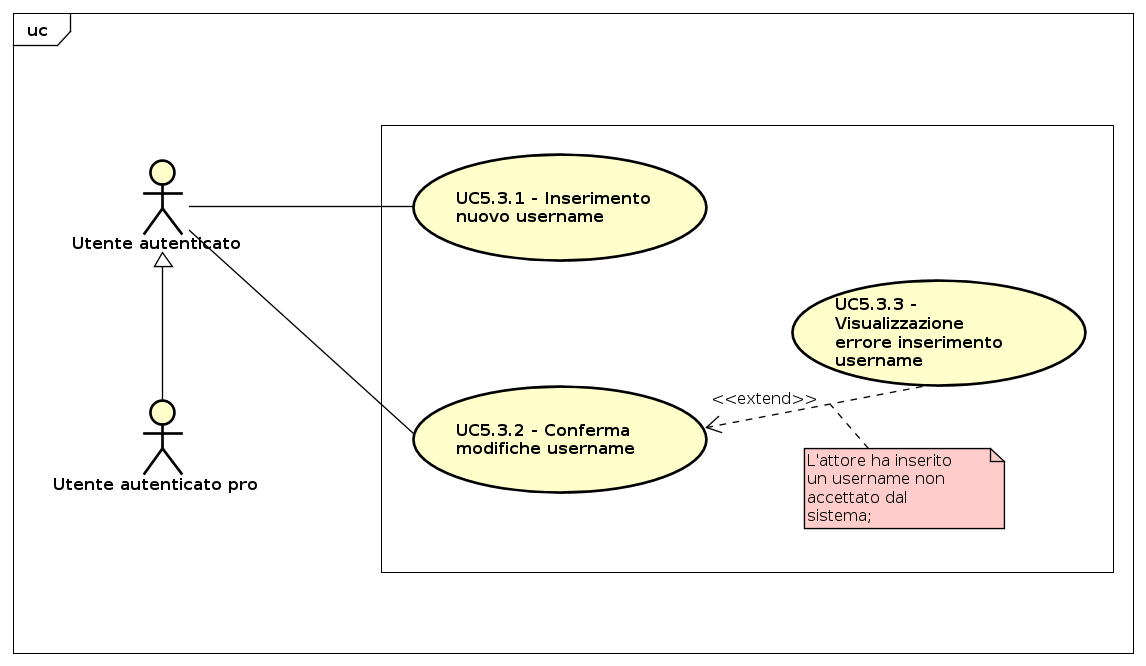
\includegraphics[scale=0.5]{UML/UC5_3.png}
\end{center}

\begin{itemize}
	\item \textbf{Attori}: utente autenticato;
	\item \textbf{Descrizione}: l'utente autenticato può modificare la propria password elettronica inserendone una nuova;
	\item \textbf{Precondizione}: il sistema presenta la schermata dove è possibile modificare la propria password;
	\item \textbf{Postcondizione}: il sistema ha reso persistenti le modifiche alla propria password;
	\item \textbf{Scenario principale}:
	\begin{enumerate}
		\item L'utente autenticato può inserire la propria vecchia password (UC5.3.1);
		\item L'utente autenticato può inserire una nuova password (UC5.3.2);
		\item L'utente autenticato può confermare la modifica della password (UC5.3.3).
	\end{enumerate}
	\item \textbf{Scenari alternativi}: l'utente autenticato annulla le modifiche e il sistema lo riporta alla schermata di gestione del profilo utente.
\end{itemize}

\paragraph{Caso d'uso UC5.3.1: Inserimento vecchia password}

\begin{itemize}
	\item \textbf{Attori}: utente autenticato;
	\item \textbf{Descrizione}: l'utente autenticato può inserire la vecchia password;
	\item \textbf{Precondizione}: il sistema richiede all'utente di inserire la vecchia password;
	\item \textbf{Postcondizione}: l'utente autenticato ha inserito la vecchia password;
	\item \textbf{Scenario principale}: l'utente autenticato inserisce la vecchia password.
\end{itemize}

\paragraph{Caso d'uso UC5.3.2: Inserimento nuova password}

\begin{itemize}
	\item \textbf{Attori}: utente autenticato;
	\item \textbf{Descrizione}: l'utente autenticato può inserire la nuova password;
	\item \textbf{Precondizione}: il sistema richiede all'utente di inserire la nuova password;
	\item \textbf{Postcondizione}: l'utente autenticato inserisce la nuova password;
	\item \textbf{Scenario principale}: l'utente autenticato inserisce la nuova password.
\end{itemize}

\paragraph{Caso d'uso UC5.3.3: Conferma modifica password}

\begin{itemize}
	\item \textbf{Attori}: utente autenticato;
	\item \textbf{Descrizione}: l'utente autenticato può confermare le modifiche alla password effettuate;
	\item \textbf{Precondizione}: l'utente ha inserito una nuova password;
	\item \textbf{Postcondizione}: il sistema rende persistenti le modifiche effettuate alla password;
	\item \textbf{Scenario principale}: l'utente conferma le modifiche alla password effettuate.
\end{itemize}

\subsubsection{Caso d'uso UC5.4: Eliminazione account}
\begin{center}
	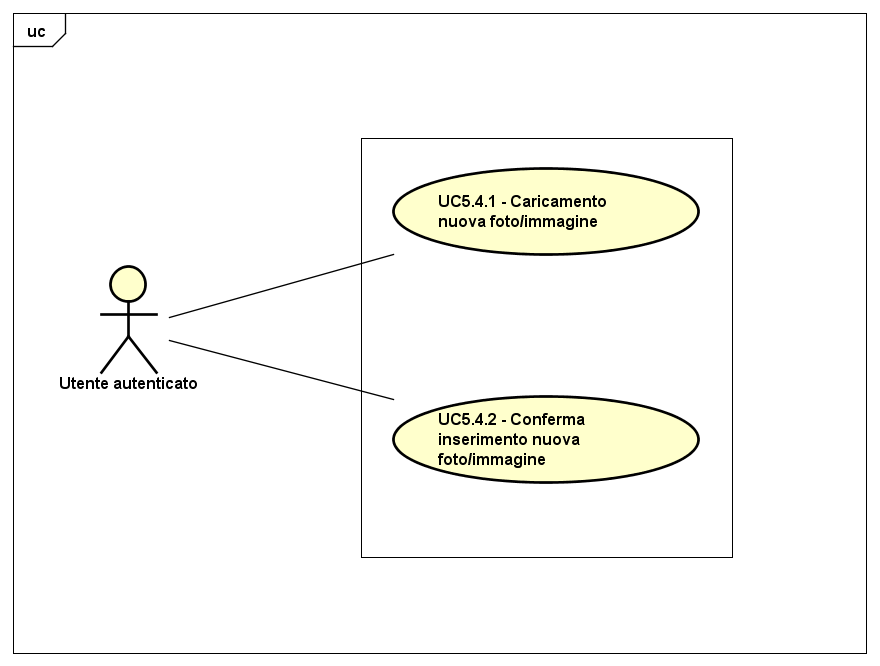
\includegraphics[scale=0.5]{UML/UC5_4.png}
\end{center}

\begin{itemize}
	\item \textbf{Attori}: utente autenticato;
	\item \textbf{Descrizione}: l'utente autenticato può eliminare il proprio account dal sistema; l'eliminazione dell'account comporta la cancellazione dei propri dati dal sistema; 
	\item \textbf{Precondizione}: il sistema visualizza l'opzione dove è possibile eliminare il proprio account;
	\item \textbf{Postcondizione}: il sistema ha eliminato in maniera persistente il proprio account e tutti i relativi dati;
	\item \textbf{Scenario principale}:
		\begin{enumerate}
			\item L'utente può confermare l'eliminazione del proprio account e dei relativi dati personali (UC5.4.1).
		\end{enumerate}
\end{itemize}

\paragraph{Caso d'uso UC5.4.1: Conferma eliminazione account}

\begin{itemize}
	\item \textbf{Attori}: utente autenticato;
	\item \textbf{Descrizione}: l'utente autenticato può confermare la cancellazione del proprio account e dei relativi dati dal sistema;
	\item \textbf{Precondizione}: l'utente ha richiesto al sistema di eliminare il proprio account;
	\item \textbf{Postcondizione}: il sistema ha eliminato l'account dell'utente richiedente e tutti i relativi dati;
	\item \textbf{Scenario principale}: l'utente conferma l'eliminazione del proprio account;
\end{itemize}